\section{Implementation and Evaluation} \label{sec:evaluation}
We implement \sysname as a fork of Mysticeti~\cite{mysticeti} and evaluate it on a geo-distributed AWS testbed. We use the same setup as the Mysticeti paper~\cite{mysticeti}\footnote{
    13 different AWS regions; \texttt{m5.8xlarge} (instances with 32 vCPUs, 128GB RAM, and 10Gbps network); 512 bytes transactions; each data point is the average latency and error bar represent one stdev; benchmarks run for multiple minutes under fixed load.
} and only test for loads up to 50k tx/s to limit costs. We set $t_a = 10\%$ and auxiliary validators propose blocks every few seconds.

\begin{figure}[t]
    \vskip -1em
    \centering
    \begin{minipage}{.58\textwidth}
        \centering
        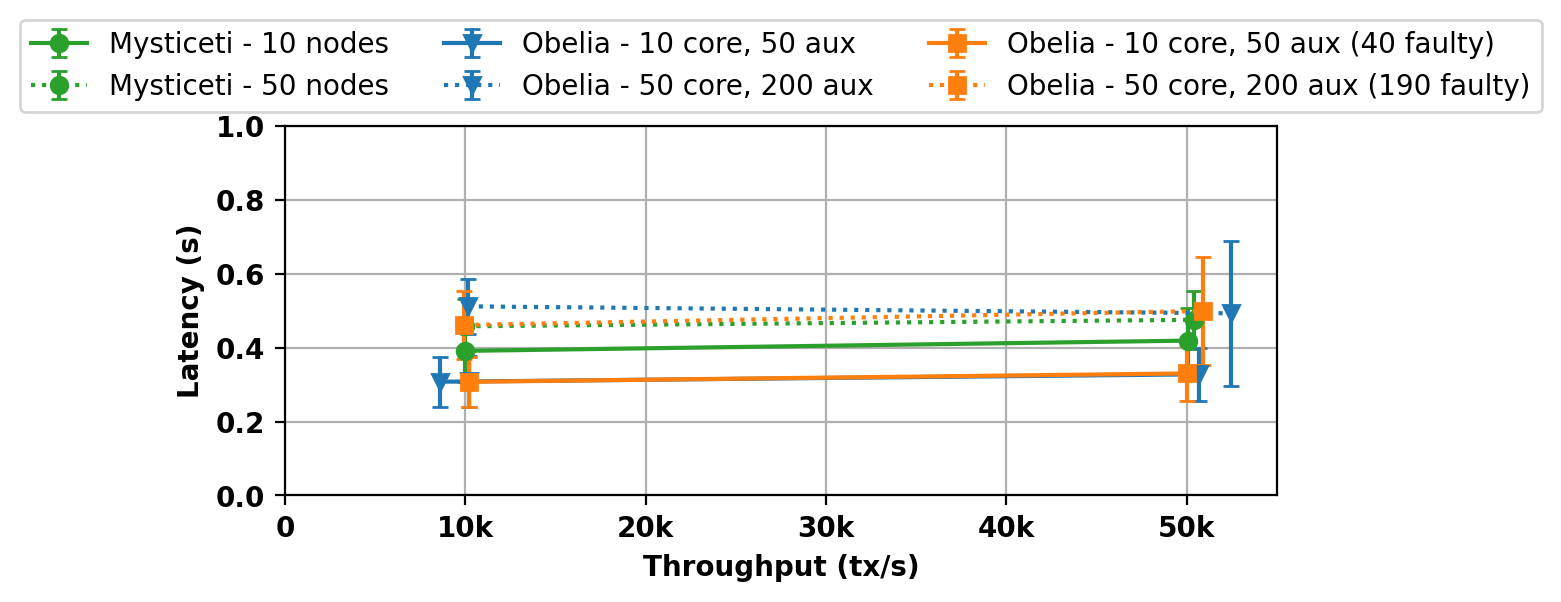
\includegraphics[width=\textwidth]{data/plots/overhead}
    \end{minipage}
    \begin{minipage}{0.38\textwidth}
        \centering
        \vfill
        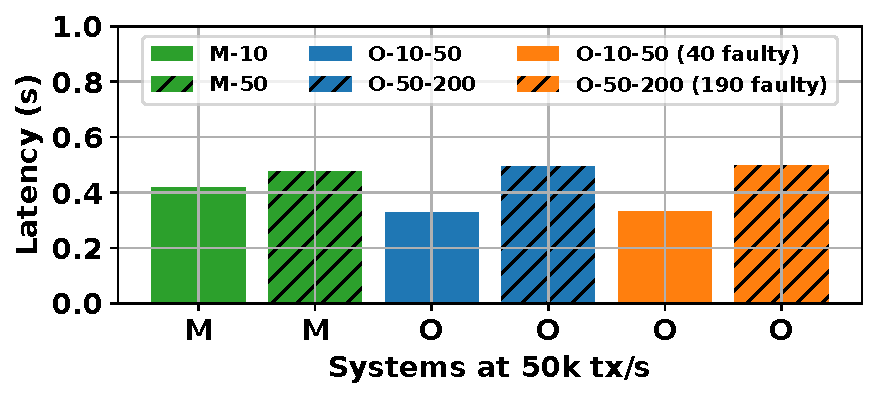
\includegraphics[width=\textwidth]{data/plots/histogram}
    \end{minipage}
    \caption{
        Comparative evaluation of Mysticeti (10 and 50 validators) and \sysname (10 core + 50 auxiliary validators, 50 core + 200 auxiliary validators). Left: throughput-latency graph. Right: Latency zoom at 50k tx/s.
    }
    \label{fig:evaluation}
    \vskip -1em
\end{figure}

Regardless of the committee size, \Cref{fig:evaluation} shows no statistical different between Mysticeti and \sysname, thus validating our claim \textbf{G4} that \sysname introduces negligible overhead. \Cref{fig:evaluation} also shows that \sysname can scale to 200 auxiliary validators, this validates our claim \textbf{G5} that \sysname can scale to hundreds of validators. \Cref{fig:evaluation} shows that even a large number of crashed auxiliary validators do not affect the performance of the core validators, this validates our claim \textbf{G6}.